\chapter{Syntactic Extraction}
\label{ch:extraction}

\section{Overview}
\label{sec:extraction_overview}

The extraction phase is the first stage of the analysis pipeline. It
transforms source code files into the language-agnostic Intermediate
Representation defined in Chapter \ref{ch:ir_formalization}.
Formally, the extraction phase is defined as:
$$\varepsilon : \mathcal{W} \to \mathcal{D}$$
where the workspace $\mathcal{W}$ represents the collection of source
files across
the repository, and $\mathcal{D}$ denotes the domain of valid module hierarchies
$\vec{\mathcal{M}}$.
For each individual source file $w \in \mathcal{W}$, extraction parses the file
using the corresponding language grammar $L \in \mathcal{L}$ and
produces a local
module hierarchy $\vec{\mathcal{M}} \in \mathcal{D}$.
This is the \textbf{only phase that depends on the source language}
$L \in \mathcal{L}$. Since Tree-sitter CST nodes contain only
positional metadata (byte offsets into the source buffer), every
extraction function accesses the underlying source buffer of $w$
to retrieve textual identifiers and expressions.

The extraction subsystem is organized into four logical layers, each
depending only on the layers below it (depicted in Figure
  \ref{fig:extraction_layers}
and summarized in Table \ref{tab:extraction_layers}):

\begin{figure}[htpb]
  \centering
  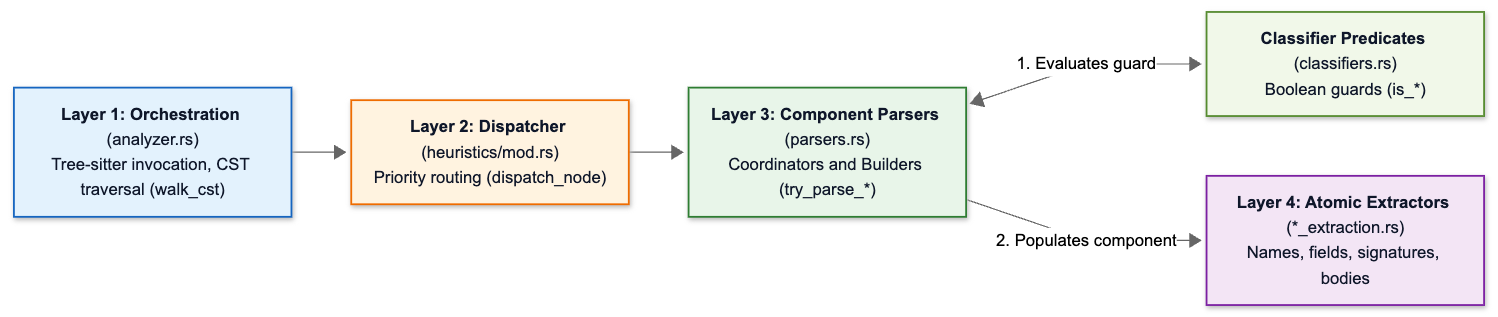
\includegraphics[width=\textwidth]{images/extraction/extraction_layers.png}
  \caption{Layered architecture of the syntactic extraction subsystem.}
  \label{fig:extraction_layers}
\end{figure}

\begin{table}[htpb]
  \centering
  \small
  \begin{tabularx}{\textwidth}{|c|>{\raggedright\arraybackslash}p{4.2cm}|>{\raggedright\arraybackslash}X|}
    \hline
    \textbf{Layer} & \textbf{Module} & \textbf{Responsibility} \\ \hline
    1 (Top) & \texttt{analyzer.rs} & Orchestration: Tree-sitter
    parsing, CST traversal, workspace grouping \\ \hline
    2 & \texttt{heuristics/mod.rs} & Dispatcher
    (\texttt{dispatch\_node}), priority routing \\ \hline
    3 & \texttt{heuristics/classifiers.rs}, \texttt{parsers.rs} &
    Classification predicates and IR component parsers \\ \hline
    4 (Bottom) & \texttt{heuristics/*\_extraction.rs},
    \texttt{text\_parsing.rs} & Low-level data extraction from CST
    nodes \\ \hline
  \end{tabularx}
  \caption{Logical layer architecture of the extraction subsystem.}
  \label{tab:extraction_layers}
\end{table}

\section{The Entry Point: \texttt{generic\_extract}}
\label{sec:generic_extract}

The top-level extraction function \texttt{generic\_extract} receives
a Tree-sitter \texttt{Language} grammar and a source string, and
produces a vector of IR modules. Its workflow is:
\begin{enumerate}
  \item A Tree-sitter parser is instantiated and configured with the
    language grammar.
  \item The source code is parsed into a Concrete Syntax Tree (CST),
    producing a root node.
  \item If the language uses package declarations (e.g., Java's
    \texttt{package com.example;}), the root children are scanned for
    a package declaration node and the package path is extracted.
  \item A module vector and a pending-attributes buffer are initialized.
  \item The recursive traversal function \texttt{walk\_cst} is
    invoked on the root node, populating the module vector with
    extracted IR components.
\end{enumerate}

The function returns both the extracted modules and the optional
package path. A higher-level function, \texttt{parse\_source}, then
applies the appropriate Module Grouping Strategy (Section
\ref{sec:module_strategies}) and loads the Primitive Registry for the language.

\section{CST Traversal: \texttt{walk\_cst}}
\label{sec:walk_cst}

The function \texttt{walk\_cst} is the core of the extraction phase.
It recursively visits every node of the CST and delegates
classification to the dispatcher. Its traversal logic follows four rules:

\begin{enumerate}
  \item For each CST node, invoke \texttt{dispatch\_node}. If the
    dispatcher returns a recognized component, insert it into the
    current module (\texttt{modules[0]}) and \textbf{return
    immediately}, without descending into children. This ``pruning''
    rule is fundamental: without it, the methods of a class would be
    extracted both as members of the class (by the structured type
    parser) and again as independent free functions (by a subsequent
    recursive call).
  \item \textbf{Exception for Modules}: When a module is recognized
    (e.g., Rust \texttt{mod}, C++ \texttt{namespace}), a temporary
    module vector containing the newly parsed module is created, and
    the children of the CST module node are re-traversed in the
    context of this new module. After traversal, the populated module
    is attached as a sub-module of \texttt{modules[0]}. This
    mechanism preserves the hierarchical nesting of the source code in the IR.
  \item \textbf{Exception for Functions}: When a free function is
    recognized, its children of type ``body'' or ``block'' are still
    traversed. This handles the case of struct or class definitions
    nested inside a function body, which is permitted in some
    languages. Components found during this secondary traversal are
    inserted into the current module, not into the function.
  \item If the dispatcher returns \texttt{None} (unrecognized node),
    recursively traverse all children of the current node.
\end{enumerate}

Figure \ref{fig:cst_pruning_flow} summarizes this traversal workflow,
highlighting the pruning branch that prevents redundant extraction of
internal methods as free functions.

\begin{figure}[htpb]
  \centering
  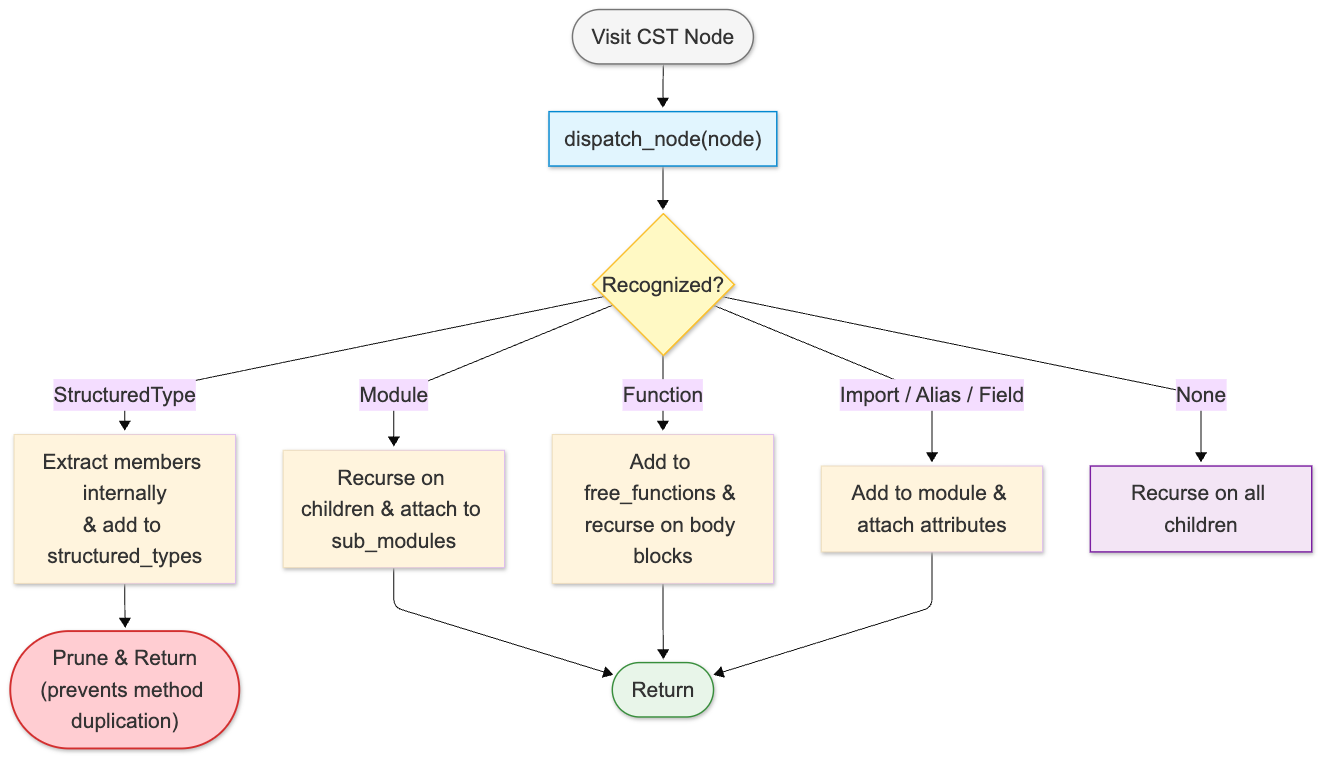
\includegraphics[width=\textwidth]{images/extraction/cst_pruning_flow.png}
  \caption{Flowchart of the \texttt{walk\_cst} traversal logic and
  subtree pruning mechanism.}
  \label{fig:cst_pruning_flow}
\end{figure}

An implicit ``root'' module is created lazily on demand: when the
first component is encountered and the module vector is still empty,
a module named \texttt{"root"} is inserted. This ensures that the IR
always contains at least one module container.

\subsection{Pending Attributes Mechanism}

Annotations and decorators (e.g., Python's \texttt{@staticmethod},
Rust's \texttt{\#[derive(Debug)]}, Java's \texttt{@Override}) are
syntactically placed \textit{before} the component they annotate. The
CST represents them as sibling nodes, not as children of the
annotated component. To handle this, \texttt{walk\_cst} maintains a
\texttt{pending\_attributes} buffer: when the dispatcher recognizes
an attribute node, the extracted annotation type references are
appended to this buffer. When the next component (function, class,
field, etc.) is recognized, the buffered attributes are attached to
it as its \texttt{annotations} list, and the buffer is cleared.

\section{The Heuristic Dispatcher}
\label{sec:dispatcher}

The dispatcher is the central decision point of the extraction phase.
For each CST node, it invokes a chain of \texttt{try\_parse\_*}
functions in a fixed priority order, returning the first successful match:

\begin{enumerate}
  \item \textbf{Imports} (highest priority): Recognized via exact
    node kind matching (\texttt{use\_declaration},
      \texttt{import\_declaration}, \texttt{import\_statement},
    \texttt{import\_from\_statement}, \texttt{preproc\_include}).
  \item \textbf{Attributes / Decorators}: Nodes of kind
    \texttt{attribute\_item}, \texttt{decorator}, or similar are
    recognized and their contents extracted into type references,
    returning a \texttt{ParsedItem::Attribute}.
  \item \textbf{Modules / Namespaces}: Recognized only if the
    language configuration enables \texttt{inline\_mod\_based} or
    \texttt{namespace\_based} modules (e.g., Rust \texttt{mod
    \{...\}}, C++ \texttt{namespace \{...\}}).
  \item \textbf{Structured Types}: Classes, structs, interfaces,
    traits, enums, and enum variants.
  \item \textbf{Functions / Methods}: Free functions, method
    declarations, constructors, and Python
    \texttt{decorated\_definition} wrappers.
  \item \textbf{Implementation Blocks}: Rust \texttt{impl} items
    (only if \texttt{support\_impl\_blocks} is enabled).
  \item \textbf{Type Aliases}: \texttt{typedef},
    \texttt{type\_alias\_declaration}, \texttt{type\_item}, and
    related node kinds.
  \item \textbf{Free Variables / Global Declarations} (lowest
    priority): Static items, const items, and top-level variable declarations.
\end{enumerate}

The dispatch order prevents ambiguity: a module node must be captured
as a module before any of its inner structs are individually matched,
and a class node must be captured as a whole before its methods are
matched as free functions. This ordering is critical for correctness.

The dispatcher's return type is a \texttt{ParsedItem} enum with four
variants: \texttt{Component} (for modules, types, functions, fields,
type aliases), \texttt{ImplBlock}, \texttt{Imports} (which may return
multiple imports from a single node), and \texttt{Attribute}.

\section{Classification Heuristics}
\label{sec:classifiers}

The classifiers are boolean predicates that identify the
\textit{role} of a CST node. They use string-based pattern matching
on the node's \texttt{kind()} property. This approach is the key to
language agnosticism: rather than maintaining separate grammar rules
per language, the analyzer exploits the fact that Tree-sitter
grammars across different languages use similar naming conventions
for equivalent constructs \cite{brunsfeld_treesitter_2018}.
In contrast to universal syntax tree frameworks such as Babelfish
UAST \cite{babelfish_uast},
which attempt to map diverse languages into a single unified
taxonomy, OmniDeps relies
on lightweight nominal heuristics directly over native CST nodes.

Each classifier follows a pattern of \textbf{positive conditions} (the
  node kind must match or contain expected substrings, or satisfy structural
sub-tree patterns) combined with \textbf{negative exclusions} (the node kind
or syntactic context must \textit{not} indicate a different semantic role).

\begin{table}[htpb]
  \centering
  \footnotesize
  \begin{tabularx}{\textwidth}{|l|>{\raggedright\arraybackslash}X|>{\raggedright\arraybackslash}X|}
    \hline
    \textbf{Classifier} & \textbf{Positive Conditions} &
    \textbf{Negative Exclusions} \\ \hline
    \texttt{is\_module} & \texttt{mod\_item}, \texttt{module},
    \texttt{namespace} & \texttt{identifier} \\ \hline
    \texttt{is\_package\_declaration} & \texttt{package\_declaration},
    \texttt{package\_clause} & None (exact match) \\ \hline
    \texttt{is\_structured\_type} & \texttt{struct}, \texttt{class},
    \texttt{interface}, \texttt{trait}, \texttt{enum}, \texttt{union},
    \texttt{annotation\_type}; or \texttt{type\_definition} enclosing
    \texttt{struct}, \texttt{enum}, or \texttt{union} &
    \texttt{bound}, \texttt{clause}, \texttt{list}, \texttt{expression},
    \texttt{argument}, \texttt{call}, \texttt{identifier},
    \texttt{reference}, \texttt{body}, \texttt{mod}, \texttt{super},
    \texttt{base}, \texttt{constructor} \\ \hline
    \texttt{is\_function} & \texttt{function}, \texttt{method},
    \texttt{fn\_item}, \texttt{func}, \texttt{constructor},
    \texttt{decorated\_definition}; or \texttt{declaration} with nested
    \texttt{function\_declarator} & \texttt{class} \\ \hline
    \texttt{is\_import} & \texttt{use\_declaration},
    \texttt{import\_declaration},
    \texttt{import\_statement}, \texttt{import\_from\_statement},
    \texttt{preproc\_include} & None (exact match) \\ \hline
    \texttt{is\_impl\_block} & \texttt{impl\_item},
    \texttt{impl\_block} & None \\ \hline
    \texttt{is\_free\_variable} & \texttt{static\_item}, \texttt{const\_item},
    \texttt{global\_variable\_declaration}; or top-level \texttt{declaration},
    \texttt{variable\_declaration} & Ancestor is function, method,
    body, or block scope;
    or contains nested \texttt{function\_declarator} \\ \hline
    \texttt{is\_type\_alias} & \texttt{type\_alias\_declaration},
    \texttt{alias\_declaration},
    \texttt{type\_item}, \texttt{type\_alias\_statement}; or non-struct
    \texttt{type\_definition} & Excludes structured types \\ \hline
  \end{tabularx}
  \caption{Summary of classifier predicates and their heuristic matching rules.}
  \label{tab:classifiers}
\end{table}

The negative exclusions are necessary to prevent false positives.
Some representative examples:
\begin{itemize}
  \item \texttt{struct\_expression} contains ``struct'' but
    represents a struct instantiation (e.g., \texttt{MyStruct \{
    field: value \}}), not a type definition. The exclusion of
    ``expression'' prevents this from being classified as a structured type.
  \item \texttt{constructor\_declaration} contains ``struct'' (via
    ``con\textbf{struct}or'') and must be excluded.
  \item \texttt{class\_body} contains ``class'' but is the body of a
    class, not the class declaration itself. The exclusion of
    ``body'' prevents this match.
  \item \texttt{trait\_bound} and \texttt{base\_class\_clause}
    contain ``trait'' and ``class'' respectively, but represent
    constraint syntax, not type definitions.
\end{itemize}

The \texttt{is\_import} classifier is the only one that uses exact
matching (\texttt{matches!} in Rust) rather than substring
containment, because import node names are highly specific and
substring matching would cause excessive false positives.

The \texttt{is\_free\_variable} classifier is notable for its use of
\textbf{parent chain inspection}: in C, both global and local
variable declarations produce the same \texttt{declaration} node
kind. To distinguish them, the classifier walks up the parent chain.
If the declaration is nested inside a \texttt{compound\_statement} or
\texttt{function\_definition}, it is classified as local (and
ignored); if its parent is a \texttt{translation\_unit} or
\texttt{declaration\_list}, it is classified as a global variable.

A specialized helper, \texttt{has\_nested\_function\_declarator},
unrolls nested C/C++ declarators to disambiguate function
declarations from variable declarations that happen to contain
function pointer syntax.

\section{Structural Parsers}
\label{sec:parsers}

Rather than processing nodes in a rigid sequential pipeline, the extraction
subsystem adopts a coordinator pattern. The heuristic dispatcher
delegates candidate nodes to the structural parsers (\texttt{try\_parse\_*}).
Each parser coordinates the extraction of a specific component kind: it first
invokes the corresponding classifier predicate as a boolean guard to verify
whether the CST node matches the target role. If the check succeeds, the parser
coordinates the lower-level atomic extractors to retrieve identifiers, fields,
signatures, and method bodies, assembling and returning the populated IR
component. If the classifier returns false, the parser immediately returns
\texttt{None}, prompting the dispatcher to evaluate the next candidate.

\subsection{Structured Type Parsing}

The \texttt{try\_parse\_structured\_type} function extracts the full
content of a class, struct, interface, trait, or enum definition:
\begin{enumerate}
  \item The qualified name is extracted via \texttt{extract\_qualified\_name}.
  \item The \texttt{StructuredTypeKind} is determined by inspecting
    the node kind and its textual content (\texttt{Class},
      \texttt{Struct}, \texttt{Interface}, \texttt{Trait},
    \texttt{Enum}, \texttt{EnumVariant}).
  \item Fields, methods, super-types, nested types, and annotations
    are extracted using the respective extractors.
\end{enumerate}

A special case handles C/C++ \texttt{type\_definition} nodes that
contain an inner \texttt{struct\_specifier} or
\texttt{enum\_specifier}: the parser hoists the fields from the inner
specifier and filters out redundant anonymous types.

The methods, fields, and nested types are extracted
\textit{internally} by the structured type parser, using the generic
list combinator \texttt{extract\_list\_of}. This is why the CST
traversal in \texttt{walk\_cst} prunes the subtree after recognizing
a structured type: all relevant information has already been
extracted by the parser.

\subsection{Function Parsing}

The \texttt{try\_parse\_function} function extracts:
\begin{enumerate}
  \item The identifier (with special handling for Python's
    \texttt{decorated\_definition}, which wraps the actual function definition).
  \item Parameters, via \texttt{extract\_parameters}.
  \item The return type, via \texttt{extract\_return\_type}.
  \item The \texttt{is\_constructor} flag, set to \texttt{true} if
    the node kind contains ``constructor''.
  \item Annotations, via the annotation extraction module.
  \item The function body, if present: the parser looks for a child
    named \texttt{"body"}, or falls back to children of kind
    \texttt{"block"}, \texttt{"constructor\_body"}, or
    \texttt{"statement\_block"}. If found, the body is extracted as a
    structured \texttt{Block} ($\mathcal{B}$) via
    \texttt{extract\_block} (Section \ref{sec:body_extraction}). If
    no body is found (e.g., forward declarations in C/C++ headers),
    the body is set to \texttt{None}.
\end{enumerate}

\subsection{Import Parsing}

The \texttt{try\_parse\_imports} function handles import statements
across all supported languages. It returns a vector of
\texttt{Import} structures because some syntactic forms (e.g.,
Python's \texttt{from module import a, b, c}) produce multiple
logical imports from a single CST node. The parser:
\begin{itemize}
  \item Detects wildcard imports by checking for \texttt{*},
    \texttt{.*}, \texttt{::*}, or \texttt{using namespace} patterns.
  \item Detects import aliases by searching for the \texttt{as}
    keyword in the import text.
  \item Extracts import paths using CST named fields where available,
    with textual fallback parsing. File extensions (e.g.,
    \texttt{.h}, \texttt{.hpp}) are stripped from C/C++
    \texttt{\#include} paths.
\end{itemize}

\subsection{Implementation Block Parsing}

The \texttt{try\_parse\_impl\_block} function extracts:
\begin{itemize}
  \item The target type (\texttt{impl\_for}), as a \texttt{TypeRef}.
  \item The optionally implemented trait
    (\texttt{implements\_trait}), extracted by searching for the
    \texttt{for} keyword in the node text to distinguish \texttt{impl
    Type} from \texttt{impl Trait for Type}.
  \item Methods, nested types, and type aliases defined within the block.
\end{itemize}

\subsection{Type Alias and Free Variable Parsing}

Type aliases are extracted with their name and target type reference.
Free variables (global constants, static items) are extracted as
\texttt{Field} entries with their name, type reference, and annotations.

\section{Low-Level Extractors}
\label{sec:extractors}

The lowest layer of the extraction subsystem provides atomic
functions that interact directly with CST nodes.

\subsection{Text Extraction}

\begin{itemize}
  \item \textbf{\texttt{node\_text}}: Extracts the raw source text
    corresponding to a CST node by reading from the source buffer
    using the node's byte range. This is the fundamental bridge
    between the positional CST and the textual content of the source code.
  \item \textbf{\texttt{split\_qualified\_name}}: Normalizes a
    qualified name string (e.g., \texttt{std::vec::Vec},
    \texttt{java.util.List}) into a \texttt{QualifiedName} vector by
    splitting on separator characters (\texttt{:}, \texttt{.}, and
    whitespace). The \texttt{->} operator is normalized to \texttt{.}
    before splitting, and generic type arguments (\texttt{<...>}) are stripped.
\end{itemize}

\subsection{Identifier Extraction}

\begin{itemize}
  \item \textbf{\texttt{extract\_identifier}}: Extracts the simple
    name of a component by trying a chain of named fields
    (\texttt{name}, \texttt{type\_identifier}, \texttt{identifier}),
    with a fallback to the \texttt{declarator} field for C/C++
    declarations. The declarator fallback recursively descends nested
    declarator nodes (\texttt{pointer\_declarator},
    \texttt{function\_declarator}) to reach the base identifier.
  \item \textbf{\texttt{extract\_qualified\_name}}: Extracts
    multi-part names by first trying named fields and applying
    \texttt{split\_qualified\_name}, then falling back to collecting
    all child nodes of type \texttt{identifier} or
    \texttt{type\_identifier} into a vector.
\end{itemize}

\subsection{Type Reference Extraction}

The function \texttt{extract\_type\_ref} converts a CST node into a
\texttt{TypeRef}. It operates through a cascade of progressively less
specific strategies:

\begin{enumerate}
  \item \textbf{Direct identifiers}: If the node itself is an
    \texttt{identifier}, \texttt{type\_identifier},
    \texttt{scoped\_identifier}, \texttt{field\_access}, or
    \texttt{attribute}, its text is extracted directly and split into
    a qualified name. This is the most reliable path.
  \item \textbf{Union types}: If the node represents a union type
    (\texttt{union\_type}, a binary operator with \texttt{|}, or a
    \texttt{Union[...]} annotation), it is recursively decomposed
    into \texttt{TypeRef::Union($\vec{\tau}$)} to represent type disjunctions.
  \item \textbf{Named fields}: The node's children are inspected for
    named fields \texttt{type}, \texttt{return\_type},
    \texttt{field\_type}, \texttt{value\_type}, and \texttt{right}.
    If found, the field's text is split into a qualified name.
  \item \textbf{Child identifier search}: All children are iterated,
    looking for nodes of kind \texttt{type\_identifier},
    \texttt{primitive\_type}, \texttt{identifier}, or \texttt{type}.
    A guard rejects children whose text contains whitespace, to avoid
    capturing complex expressions.
  \item \textbf{Textual fallback}: The node text is scanned for
    \texttt{:} or \texttt{->} characters, and everything after the
    delimiter is taken as the type name.
  \item \textbf{Failure}: If all strategies fail,
    \texttt{TypeRef::Failed(vec![])} is returned.
\end{enumerate}

\subsection{Parameter Extraction}

The function \texttt{extract\_parameters} locates the
\texttt{parameters} named field and iterates over its children of
type ``parameter''. For each parameter, it extracts:
\begin{itemize}
  \item The parameter name via \texttt{extract\_identifier}.
  \item The parameter type via \texttt{extract\_type\_ref}.
  \item The variadic flag, set to \texttt{true} if the parameter text
    contains \texttt{...} or \texttt{*args}.
\end{itemize}

A \textbf{sanitization step} is applied to prevent a common false
positive in dynamically typed languages: if the extracted type text
matches the parameter name exactly (e.g., \texttt{self} in Python,
where the parameter has no type annotation), the extractor recognizes
that the fallback captured the parameter name instead of a type, and
replaces the result with \texttt{TypeRef::Failed}. This prevents
untyped parameters from generating spurious dependencies.

\subsection{Super-Type Extraction}

The function \texttt{extract\_super\_types} searches for inheritance
references in a variety of named fields across languages:
\begin{itemize}
  \item Java: \texttt{super\_type}, \texttt{extends},
    \texttt{implements}, \texttt{interfaces}
  \item Python: \texttt{superclass}, \texttt{superclasses}
  \item C++: \texttt{base\_class\_clause} child nodes
  \item Rust: trait bounds in type parameter lists
\end{itemize}

For each found node, it traverses the children looking for
\texttt{type\_identifier}, \texttt{identifier},
\texttt{scoped\_type\_identifier}, and type lists, extracting each as
a \texttt{TypeRef::Unresolved}.

\subsection{The Generic List Combinator}

The function \texttt{extract\_list\_of<T, F>} is a higher-order
combinator that takes a parser function \texttt{F} and applies it to
all children of a node. If a child is not matched by the parser but
is a container node (its kind contains ``body'', ``list'', ``block'',
or ``declaration''), the combinator descends recursively into that container.

A guard condition prevents descent into function bodies: this ensures
that when extracting fields of a class, local variable declarations
inside methods are not mistakenly extracted as class fields. This
combinator is used to implement:
\begin{itemize}
  \item \texttt{extract\_fields}: Extracts field declarations using
    an inline field parser.
  \item \texttt{extract\_methods}: Extracts methods using
    \texttt{try\_parse\_function}.
  \item \texttt{extract\_nested\_types}: Extracts nested type
    definitions using \texttt{try\_parse\_structured\_type}.
\end{itemize}

\section{Structured Body Extraction}
\label{sec:body_extraction}

The body of a function is extracted into a structured \texttt{Block}
($\mathcal{B}$) that preserves the lexical scope hierarchy. The
function \texttt{extract\_block} classifies each child of a body node
into three categories:

\begin{enumerate}
  \item \textbf{Local Variable Declarations}: Nodes matching known
    declaration kinds (\texttt{let\_declaration},
      \texttt{local\_variable\_declaration},
      \texttt{variable\_declaration}, \texttt{lexical\_declaration},
    etc.) are extracted as \texttt{Field} entries in the block's
    \texttt{declarations} vector. When a variable has no explicit
    type annotation, the function \texttt{infer\_variable\_type}
    inspects the initializer expression for patterns that reveal the type:
    \begin{itemize}
      \item \texttt{new Foo()} or \texttt{Foo \{...\}} $\to$ the type
        is inferred as \texttt{Foo}.
      \item \texttt{Bar::new()} $\to$ the type is inferred as the
        return type of \texttt{Bar::new}, encoded as a
        \texttt{ResolutionQuery(Call(Extract(Find(Bar), new)))}.
      \item In dynamically typed code lacking type annotations \cite{pep484},
        untyped assignments like \texttt{x = Admin()} produce a
        \texttt{Query::Call} to resolve the callable's return type.
    \end{itemize}

    This mechanism highlights the modular decoupling between
    extraction ($\varepsilon$)
    and resolution ($\rho$): because per-file extraction operates
    strictly on local
    syntax without global symbol visibility,
    \texttt{infer\_variable\_type} does not
    attempt to evaluate return types eagerly. Instead, it synthesizes a deferred
    expression $q \in \mathcal{Q}$ within the Query Algebra (Chapter
    \ref{ch:ir_formalization}),
    delegating its semantic evaluation to the name resolution engine
    $\rho_{\text{exec}}$
    (Chapter \ref{ch:name_resolution}) once the global workspace
    scope tree is constructed.

  \item \textbf{Nested Blocks}: Children whose kind contains ``body''
    or ``block'', or equals \texttt{compound\_statement}, are
    recursively extracted as sub-blocks via a recursive call to
    \texttt{extract\_block}. This creates a tree of \texttt{Block}
    structures that mirrors the control-flow nesting of the source
    code (\texttt{if}, \texttt{while}, \texttt{for},
    \texttt{try/catch}, anonymous scopes).

  \item \textbf{Behavioral Dependencies}: All remaining children
    (expression statements, return statements, assignments, etc.) are
    inspected recursively to discover behavioral dependencies across four
    semantic categories:
    \begin{itemize}
      \item \textbf{Instantiations}: Constructor invocations (e.g., \texttt{new}
        expressions in Java and C++) and struct literal expressions
        (e.g., Rust struct initializations).
      \item \textbf{Function and Method Calls}: Invocations across
        three structural forms:
        \begin{itemize}
          \item \textit{Scoped calls} (\texttt{Module::func()}) $\to$
            the scope qualifier is captured to resolve namespaced or
            static calls.
          \item \textit{Method invocations} (\texttt{obj.method()})
            $\to$ the receiver object expression is captured to track
            member dereferencing.
          \item \textit{Simple calls} (\texttt{func()}) $\to$ the
            bare callable identifier is captured.
        \end{itemize}
      \item \textbf{Field and Member Accesses}: Explicit property
        accesses, attribute dereferences, and qualified symbol paths.
      \item \textbf{Type Casts}: Explicit type conversions and cast
        expressions, ensuring dependency tracking on target coercion types.
    \end{itemize}
\end{enumerate}

The behavioral dependency search \textbf{skips} nested block nodes to
avoid double-counting: dependencies inside sub-blocks are captured by
the recursive \texttt{extract\_block} call, not by
\texttt{find\_behavioral\_deps}. This guarantees that each dependency
is recorded at the exact lexical scope level where it occurs.

For Rust macros (e.g., \texttt{println!}, \texttt{vec!}), a
specialized function \texttt{parse\_token\_tree\_macro} implements a
state machine over the flat token stream to
reconstruct qualified paths and extract dependencies from macro invocations.

\section{Annotation and Decorator Extraction}
\label{sec:annotation_extraction}

Metadata annotations, decorators, and compiler attributes represent declarative
dependencies that alter runtime behavior or generate code. The
extractor captures
these dependencies across the diverse syntactic conventions of each language:

\begin{itemize}
  \item \textbf{Python}: Decorators attached to function or class definitions
    are extracted to capture meta-programming wrappers. The extractor
    handles bare
    decorators (\texttt{@decorator}), qualified module paths
    (\texttt{@module.decorator}),
    and parameterized factory calls (\texttt{@decorator(args)}).
  \item \textbf{Rust}: Outer and inner attributes associated with
    items are captured.
    In particular, derive macros (e.g., \texttt{\#[derive(Debug,
    Clone)]}) are expanded
    into individual type references, creating explicit dependencies
    on each derived trait.
  \item \textbf{Java}: Class-, method-, and field-level annotations
    (both marker and
    value-carrying annotations) are extracted, normalizing the
    annotation identifier by
    stripping leading syntactical delimiters.
  \item \textbf{C/C++}: Standard and compiler-specific attribute
    specifiers (such as
    standard \texttt{[[...]]} attributes or compiler pragmas) are
    captured when attached
    to declarations.
\end{itemize}

As described in Section \ref{sec:walk_cst}, because annotations
frequently appear syntactically
before their target construct rather than inside its subtree,
extracted annotations are
buffered during CST traversal and attached to the subsequent
recognized component.

\section{Dynamic Field Extraction}
\label{sec:dynamic_fields}

In Python, instance fields are typically not declared at the class
level but are dynamically assigned in methods via \texttt{self.field
= value} patterns. When the \texttt{extract\_dynamic\_fields}
configuration flag is enabled, the field extractor enters method
bodies and tracks the active \texttt{self} parameter name.
Assignments to \texttt{self.field} are detected and the field name
and inferred type are extracted. Field types are inferred from the
right-hand side of the assignment using \texttt{infer\_variable\_type}.

To prevent duplicates when a field is assigned in multiple methods,
the extractor deduplicates fields by name, favoring entries with more
informative type references (resolved or inferred types over
unresolved or failed ones).

\section{Language-Agnostic Structural Heuristics}
\label{sec:structural_heuristics}

The extraction layer relies on heuristics that operate purely on CST
structure without language-specific branches:

\begin{itemize}
  \item \textbf{Recursive Declarator Descent}: In C and C++, the base
    identifier or parameter list of a function declaration can be
    nested inside multiple declarator nodes (e.g.,
      \texttt{pointer\_declarator} wrapping
    \texttt{function\_declarator}). The extractors recursively
    descend the CST until they identify the semantic leaf, enabling
    correct extraction of functions returning pointers, typedefs, and
    complex declaration forms. The helper
    \texttt{has\_nested\_function\_declarator} assists in
    distinguishing function declarations from pointer variable declarations.

  \item \textbf{Contextual Classification via Parent Chain}: To
    distinguish global from local variables when they share the same
    node kind (\texttt{declaration} in C), the classifier inspects
    ancestor nodes. Declarations nested inside a
    \texttt{compound\_statement} or \texttt{function\_definition} are
    classified as local; those under a \texttt{translation\_unit} are
    classified as global.

  \item \textbf{C \texttt{type\_definition} Hoisting}: C's
    \texttt{typedef struct \{...\} Name;} pattern produces a
    \texttt{type\_definition} node containing an inner
    \texttt{struct\_specifier}. The parser detects this pattern,
    hoists the inner fields from the specifier, assigns the outer
    name, and produces a single \texttt{StructuredType} without a
    redundant anonymous inner type.
\end{itemize}

\section{Workspace Orchestration}
\label{sec:workspace_orchestration}

While \texttt{generic\_extract} operates on individual files, the
analyzer is designed for multi-file projects. The workspace
orchestration proceeds as follows:

\begin{enumerate}
  \item The workspace directory is recursively scanned using
    \texttt{walkdir}. Files are filtered by extension to determine
    the source language (\texttt{.rs}, \texttt{.java}, \texttt{.py},
    \texttt{.c}, \texttt{.cpp}, \texttt{.h}, \texttt{.hpp}, etc.).
  \item Each file is independently extracted via
    \texttt{parse\_source}, which invokes \texttt{generic\_extract}
    and then applies the Module Grouping Strategy.
  \item All extracted module hierarchies are accumulated into the
    global module hierarchy $\vec{\mathcal{M}} \in \mathcal{D}$. Primitive
    registries from each language are merged into a combined registry.
  \item Only after all files have been extracted and unified does the
    system invoke the subsequent pipeline phases. This design ensures
    that cross-file dependencies are resolved transparently.
\end{enumerate}

\subsection{Module Grouping Strategies}
\label{sec:module_strategies}

The module grouping strategy determines how the flat output of
\texttt{generic\_extract} is organized into the hierarchical module
tree. The choice of strategy is controlled by the
\texttt{ModuleConfig} section of the language configuration:

\begin{itemize}
  \item \textbf{Directory-Based} (Python, Rust): The file's relative
    path within the workspace is used to construct a nested module
    hierarchy. Common root prefixes (\texttt{src}, \texttt{lib},
    \texttt{include}) are stripped, and the file stem becomes the
    leaf module name. For example, the file
    \texttt{src/core/utils.py} produces the module path $\langle
    \texttt{core}, \texttt{utils} \rangle$.
  \item \textbf{Package-Declaration-Based} (Java): The file-level
    package statement (e.g., \texttt{package com.example.service;})
    determines the module hierarchy. File-scoped imports are
    distributed to all top-level structured types to ensure that each
    class carries its own import context, preventing cross-class import leakage.
  \item \textbf{Namespace / Inline Module} (C++, Rust): Namespace or
    inline module blocks are parsed during CST traversal and directly
    create sub-modules in the IR tree. No post-hoc grouping is needed.
  \item \textbf{Flat / Fallback} (C): All components are placed into
    a single root module.
\end{itemize}

Table \ref{tab:module_strategies} summarizes the strategy assignment
for each supported language.

\begin{table}[htpb]
  \centering
  \small
  \begin{tabular}{|l|c|c|c|c|c|}
    \hline
    \textbf{Grouping Strategy} & \textbf{Python} & \textbf{Rust} &
    \textbf{Java} & \textbf{C++} & \textbf{C} \\ \hline
    File-Based & \checkmark & \checkmark & & & \\ \hline
    Directory-Based & \checkmark & \checkmark & & & \\ \hline
    Package-Declaration & & & \checkmark & & \\ \hline
    Namespace & & & & \checkmark & \\ \hline
    Inline Module & & \checkmark & & & \\ \hline
    Flat (Root Module Only) & & & & & \checkmark \\ \hline
  \end{tabular}
  \caption{Module grouping strategy assignment for each supported language.}
  \label{tab:module_strategies}
\end{table}

\subsection{Out-of-Line Method Linking}
\label{sec:out_of_line}

In C++, methods are frequently declared inside a class header
(\texttt{.hpp}) and defined out-of-line in a separate source file
(\texttt{.cpp}) using qualified names (e.g., \texttt{void
MyClass::myMethod() \{ ... \}}). Since extraction processes files
independently, these definitions are initially extracted as free
functions with multi-part qualified names.

When the \texttt{forward\_declarations} flag is enabled, the function
\texttt{link\_out\_of\_line\_methods} performs a post-extraction linking step:

\begin{enumerate}
  \item Free functions with qualified names (names containing more
    than one segment) are identified and removed from the module's
    free function list.
  \item For each such function, the class prefix is extracted and
    matched against the structured types in the current module.
  \item If the target class is found in the same module, the method
    is stripped of its class prefix and appended to the class's method list.
  \item If the target class is not found (because the declaration and
    definition are in separate files), a synthetic \texttt{ImplBlock}
    is created with the target type set to a
    \texttt{ResolutionQuery(Find(ClassName))}. This defers the
    linking to Phase 2, where the name resolution engine will locate
    the class across file boundaries.
  \item The process is applied recursively to all sub-modules.
\end{enumerate}

This approach unifies the handling of Rust \texttt{impl} blocks and
C++ out-of-line methods under the same \texttt{ImplBlock}
abstraction, reinforcing the language-agnostic design of the system.
